\documentclass{deimj}
\usepackage[dvipdfmx]{graphicx}
\usepackage[ipaex]{pxchfon}
\usepackage[hyphens]{url}
\usepackage{tabularx}
\usepackage{multirow}
\usepackage{otf}

% 印刷位置調整 %
% 必要に応じて値を変更してください.
\hoffset -10mm % <-- 左に 10mm 移動
\voffset -10mm % <-- 上に 10mm 移動

\newcommand{\AmSLaTeX}{%
$\mathcal A$\lower.4ex\hbox{$\!\mathcal M\!$}$\mathcal S$-\LaTeX}
\newcommand{\PS}{{\scshape Post\-Script}}
\def\BibTeX{{\rmfamily B\kern-.05em{\scshape i\kern-.025em b}\kern-.08em
T\kern-.1667em\lower.7ex\hbox{E}\kern-.125em X}}

\papernumber{DEIM Forum 2020 XX-YY}

\jtitle{観光地検索システムの説明性向上のための既訪問スポットと検索結果の対応付けの詳細化}
\authorlist{%
 \authorentry[em18011@ns.kogakuin.ac.jp]{潘 健太}{KENTA HAN}{UnivN}
 \authorentry[kitayama@cc.kogakuin.ac.jp]{北山 大輔}{DAISUGE KITAYAMA}{UnivN}
 }

\affiliate[UnivN]{工学院大学大学院工学研究科情報学専攻\hskip1zw
  〒163--8677 東京都新宿区西新宿1--24--2}
 {School of Engineering,Kogakuin University\\
  1--24--2,Nisisinjyuku,Tokyo,163--8677 Japan}

\begin{document}
\pagestyle{empty}
\begin{jabstract}
近年,ユーザはWeb上の観光情報を活用して旅行計画を立てることが多くなっている.
しかし,旅行は一般的に訪れたことがないスポットに行くことが多いため,観光情報を適切に理解することは困難である.
そこで,訪問したことがある観光スポットの特徴を用いて,未訪問エリアの観光スポットを対応付けして,ユーザの未知なスポットに対する理解を支援することを提案する.
本研究では,まず,観光スポットのユーザレビューを用いてレビューベクトルを作成する.
次に,ユーザにとっての観光スポットの特徴を抽出するために,既訪問スポットレビューベクトルを用いて階層的クラスタリングを行うことによって,特徴クラスタを算出する.
また,特徴クラスタに対応する検索結果スポットレビューを用いて類似度を計算し,既訪問スポットと検索結果スポットを関連付けを行い,関連性を説明するためのキーワードを抽出する.
最後に,観光スポット間の対応関係を地図上に可視化する手法を用いて,プロトタイプシステムを構築し,既訪問スポットと検索結果スポットの説明性向上のための観光スポットの対応関係を評価する実験を行う.

\end{jabstract}

\begin{jkeyword}
観光スポット,理解支援,ユーザレビュー,階層的クラスタリング,可視化
\end{jkeyword}
\maketitle

%%%%%%%%%%%%%%%%%%%%%%%%%%%%%%%%%%%%%%%%%%
%%%%%%%%%%%%%%%%%%%%%%%%%%%%%%%%%%%%%%%%%%
\section{はじめに}
\label{sec:はじめに}
旅行先を決定するとき,旅行者は観光スポット検索サイトや観光情報に関連する書籍を見て観光スポットを選び,旅行計画を立てる.
しかし,ユーザにとって訪問したいエリアは,訪問したことがなく不慣れであることが多い.
そのため,エリア内に数多く存在する観光スポットから,自身の要求に合う観光スポットを見つけることは容易ではない.
このとき,ユーザは観光スポット検索サイトのランキングやおすすめ情報を見て観光スポットを決めることが多くなると考えられる.
ユーザの意思決定の材料の1つとして,Tripadvisor\footnote{https://www.tripadvisor.com/}やじゃらん\footnote{https://www.jalan.net/kankou/}などの観光スポット検索サイトがある.
これらのサイトには特定の観光スポットを訪問したことのあるユーザがレビューを投稿し,観光スポットに関する豊富な情報が存在している.
しかし,ユーザは検索エリアに関する事前知識がないため,どのスポットのレビューを読むべきか効率的に判断することは困難である.
そのため,さまざまな観光スポットを効果的に理解するためには,ユーザが訪問した経験のあるスポットを使って検索結果スポットと比較することは効果的と考えられる.
たとえば,日本に初めて訪れるフランス人旅行者に対し,検索結果スポットである東京の「表参道」をパリにおける「シャンゼリゼ通り」と表現すると理解しやすいであろう.
この考え方は,ユーザが以前に経験した物事を現在の物事に適用する一種の類推である\cite{Gentner}.
類推は創造的思考に貢献すると指摘されている\cite{Holyoak}.
類推に関する研究の多くは,ベースとなる学習データとターゲットとなる問題が与えられ,物事の特徴を問題の特徴にマッピングして問題を解決するもの\cite{Gick}である.

我々は,すでに既訪問スポットと検索結果スポットの対応関係を抽出する手法について取り組んでいる\cite{潘DEIM}.
しかしながら,既訪問スポットそのものがユーザの関心を表すとは限らない.
例えば,あるテーマパークに訪問したユーザでも,アトラクションに関心がある場合もあれば,キャラクターに関心がある場合も考えられる.
そこで本稿では,既訪問スポットを用いてより詳細なユーザの関心を扱う手法に取り組む.
本手法では,ユーザはすでに訪問した経験のあるスポットと未訪問エリアを入力する.
そのとき,観光スポットのユーザレビューを用いて特徴ベクトルを作成する.
次に,ユーザにとっての観光スポットの特徴を抽出するために,既訪問スポットのレビューベクトルを用いて階層的クラスタリングを行うことで,特徴クラスタを算出する.
また,特徴クラスタに対応する検索結果スポットレビューを用いて類似度を計算し,既訪問スポットと検索結果スポットを関連付けを行い,関連性を説明するためのキーワードを抽出する.
最後に,観光スポット間の対応関係を地図上に可視化する手法\cite{潘STI}を用いて,プロトタイプシステムを構築し,既訪問スポットと検索結果スポットの説明性向上のための観光スポットの対応関係を評価する実験を行う.
抽出したキーワードを提示することで,ユーザの検索結果スポットに対する理解の支援を目指す.
図\ref{fig:image}は提案手法の概念図である.

本論文の構成は下記のとおりである.
2節では,関連研究について述べる.
3節では,提案手法の概要について述べる.
4節では,検索結果スポットと既訪問スポットの対応関係による地図上の可視化手法について述べる.
5節では,クラスタ分けに関する評価について述べる.
最後に,6節では,まとめと今後の課題について述べる.

\begin{figure}[t]
  \begin{center}
    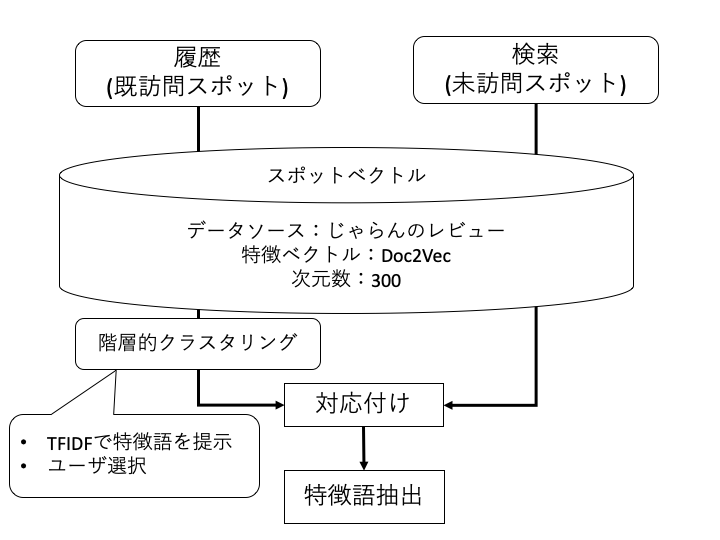
\includegraphics[clip,width=7.5cm]{picture/system_image.png}
    \caption{提案手法の概念図}
    \label{fig:image}
   \end{center}
\end{figure}


%%%%%%%%%%%%%%%%%%%%%%%%%%%%%%%%%%%%%%%%%%
%%%%%%%%%%%%%%%%%%%%%%%%%%%%%%%%%%%%%%%%%
\section{関連研究}
\label{sec:関連研究}
%%%%%%%%%%%%%%%%%%%%%%%%%%%%%%%%%%%%%%%%%%
\subsection{観光スポット検索と推薦システム}
ユーザの体験履歴を利用した検索や推薦システムに関する研究は数多く発表されている.
倉島ら\cite{Kurashima}は,Flickrに投稿された写真のジオタグ情報を人々の旅行履歴として利用した旅行ルート推薦手法を提案した.
この手法では,ユーザの現在地から行きやすい場所とユーザの興味に合致した場所に移動しやすいと仮定し,行動モデルを生成している.
ユーザのジオタグ付き写真集合は,時間情報でソートすると個人の旅行履歴とみなすことができると考え,ジオタグ情報を利用してユーザの行動モデルを生成している.
Kitamuraら\cite{Kitamura}は,一般的な物体認識を用いて,過去の個人旅行写真から推定したユーザの旅行の嗜好に基づき観光地を推薦する方法を提案した.
物体認識システムを用いて,写真で撮った被写体情報のキーワードを取得し,グラフ視覚化技術によってキーワードの共起を表現した.
また,グラフの視覚化技術に基づいて旅行写真付きのグラフを視覚化するユーザインターフェイスを紹介した.
%%%%%%%%%%%%%%%%%%%%%%%%%%%%%%%%%%%%%%%%%%
\subsection{地理的情報の可視化と意味的な関係の可視化}
本研究では,地理的情報の可視化と意味的な関係の可視化に取り組む.
地理的な情報の可視化としては,抽出した情報を地図上にマッピングするのが一般的であり,本研究もそれに従っている.
代表的な研究を以下に紹介する.
櫻川ら\cite{櫻川2015}は,ソーシャルメディア上にアップロードされた写真のジオタグ情報と撮影時刻に基づいて写真の撮影者を分類する手法を提案した.
分類された撮影者(観光者,在住者)ごとにホットスポットを可視化した.
また,ジオタグ情報と撮影時刻以外にテキストタグを加えて,写真が撮影された地域で行われるイベントの穴場スポットを発見し,地図上に提示する手法を提案した\cite{櫻川2016}.

意味的な関係性の可視化としては,グラフモデル上でオブジェクト間のつながりを関連度で表現することが多い.
上村ら\cite{上村}は,ユーザが投稿したタグ付き画像を用いたファッションスタイルの関係性の可視化手法を提案した.
ファッションスタイルは類似するタグを空間座標に固定することによって関係を表している.
本研究では,スポット間の意味的な対応関係を可視化するために,検索結果スポットは地図上で実在する座標に固定され,配置の自由があるのは既訪問スポットのみという制約がある.

%%%%%%%%%%%%%%%%%%%%%%%%%%%%%%%%%%%%%%%%%%
%%%%%%%%%%%%%%%%%%%%%%%%%%%%%%%%%%%%%%%%%
\section{検索結果スポットと既訪問スポットの対応付け}
\label{sec:検索結果スポットと既訪問スポットの対応付け}
我々は,ユーザの既訪問スポットに基づく検索結果スポットの対応付けの詳細化を提案する.
まず,ユーザがすでに訪問した複数個の観光スポットと訪問したい観光エリア情報を入力する.
本手法では,観光スポットのユーザレビューを用いて既訪問スポットのレビューベクトルを生成する.
検索結果スポットも同様にエリア内の各スポットのレビューベクトルを求める.
次に,山田ら\cite{山田}が行ったユーザの嗜好抽出手法に基づいて,ユーザの観光スポット訪問履歴から各訪問スポットに付随する個々のレビューを全て取得し,階層的クラスタリングによってレビューをクラスタに分類する.
各クラスタを正規化ジニ分散指標とスポット数で算出したスコアの上位$N$件のクラスタの特徴語をユーザに提示する.
その後,未訪問エリア内のスポットレビューを用いて,ユーザが選択したクラスタに対して平均類似度によってクラスタの分類を行う.
ユーザ選択クラスタに属する既訪問スポットと検索結果スポットのレビューベクトルの類似性によって,既訪問スポットを検索結果スポットと関連付ける.
最後に,その関係性を説明するためのキーワードを抽出する.
%%%%%%%%%%%%%%%%%%%%%%%%%%%%%%%%%%%%%%%%%%
\subsection{スポッレビューを用いたレビューベクトル生成}
本稿では,2016年9月末までのじゃらんから得られた1,481,838件のレビューデータを使用し,分散表現\cite{doc2vec}を用いてレビューベクトルの作成する.
本研究では,分散表現を計算するためにPythonのライブラリであるgensim\footnote{https://radimrehurek.com/gensim/models/doc2vec.html}を利用する.
学習方法として,Distributed Bag-of-Wordsを利用して,観光スポットのレビューを300次元のベクトルで表現する.
既訪問スポットや検索結果スポットの各レビューベクトルは,形態素解析器であるMeCab\cite{mecab}に辞書「mecab-ipadic-NEologd」\footnote{https://github.com/neologd/mecab-ipadic-neologd/}を用いて,分かち書き(原型)したレビューを利用して作成する.
%%%%%%%%%%%%%%%%%%%%%%%%%%%%%%%%%%%%%%%%%%
\subsection{既訪問スポットのクラスタ分類}
\label{sub:既訪問スポットのクラスタ分類}
本研究では,ユーザが訪れた観光スポットに,ユーザの観光スポットに対する嗜好が含まれていると仮定する.
しかし,多くの観光スポットには,単一の要素ではなく複数の要素が存在する.
そこで,山田ら\cite{山田}が行ったユーザの嗜好抽出手法に基づいて,ユーザが訪れた観光スポットに付随する全てのレビューをクラスタリングすることにより,レビューを観光スポットが持つ特徴ごとに分類する.
山田らの手法を説明する.
レビューの分類には階層的クラスタリングを利用する.
クラスタ間の距離の測定には,レビューベクトルのコサイン距離による群平均法を用いる.
群平均法とは,2つのクラスタに属する要素間の全ての組み合わせの距離を求め,その平均値をクラスタ間の距離とする手法である.
クラスタ分けの閾値は,山田らが行った実験結果により0.65とする.

階層的クラスタリングによって分類されたクラスタに対し,どのクラスタがユーザの嗜好を表しているかをスコア付けする.
本研究では,以下の条件を満たすクラスタをユーザの嗜好を表すクラスタと定義する.
\begin{itemize}
 \item 各既訪問スポットのレビューを満遍なく含んでいる
 \item より多くのスポットのレビューで構成されている
\end{itemize}

本研究では,クラスタを構成する既訪問スポットごとのレビュー数の割合を算出するため,ジニ分散指標を用いる.
ジニ分散指標とは各クラスの分散の総和を表す指標であり,クラスのばらつきが小さいと値は大きくなり,ばらつきが大きいほど値は小さくなる.
既訪問スポット数を$N$,クラスタ$c$に所属するレビューのうち,スポット$s$のレビューの割合を$P(s \mid c)$とすると,ジニ分散指標は式\ref{eq:gini}で表せる.
\begin{equation}
    gini(c)=1-\sum ^{N}_{s=1} P(s \mid c) ^{2}
    \label{eq:gini}
\end{equation}
また,各スポットのレビュー数とそのスポットの全レビュー数との割合を求めることにより,レビュー数の正規化を行なったものを正規化ジニ分散指標と呼称し,これを利用する.
スポット$s$の総レビュー数を$R_s$とすると,正規化ジニ分散指標における$P(s \mid c)$は式\ref{eq:gini_w}で表せる.
\begin{equation}
    P(s \mid c)=\frac {\frac{r_s}{R_s}}{\sum ^{N}_{j=1}\left( \frac {r_j}{R_j}\right)}
    \label{eq:gini_w}
\end{equation}

ジニ分散指標は各クラスの分散の総和のみで値が決まる関係上,クラス数までは考慮されない.
我々はより多くの既訪問スポットで構成されたクラスタが,ユーザの観光に対する嗜好を表現していると考えたため,クラスタの構成スポット数による重み付けを行う.
そのとき,あるスポットに関するレビューが1つしかない場合でも,そのクラスタを構成するスポットとしてカウントしてしまう問題がある.
そこで本研究では,クラスタを構成するあるスポットのレビュー数と,そのスポットの全レビュー数との割合が閾値以上のものを,クラスタを構成するスポットとする.
本稿では,閾値を1\%以上と決定した.

クラスタ$c$の嗜好の興味度$pref(t)$は,あるスポットに関するレビュー数の割合が閾値以上のスポット数を$s_c$とし,式\ref{eq:pref}で示す.
\begin{equation}
    pref(c)=gini(c) \times\log s_c
    \label{eq:pref}
\end{equation}
%%%%%%%%%%%%%%%%%%%%%%%%%%%%%%%%%%%%%%%%%%
\subsection{クラスタの特徴語抽出}
\label{sub:クラスタの特徴語抽出}
山田ら\cite{山田}の手法によってユーザの嗜好を表すクラスタを抽出できる.
本稿では,抽出したクラスタをユーザが任意に選択する必要がある.
そのため,各クラスタの特徴語をユーザに提示する.
各クラスタの特徴語として,スコア付されたクラスタに所属するレビューを用いて,TFIDF法で各単語のTFIDF値を求め,各クラスタの上位10件までの単語をユーザに提示する.
各単語の特徴量を式\ref{math:tfidf}で定義する.
\begin{eqnarray}
c\_word(w,c) = TF_{c}(w) \times log\frac{C}{df(w)}
    \label{math:tfidf}
\end{eqnarray}

ここで,全クラスタ数を$C$,クラスタ$c$における単語$w$の出現回数を$tf_{c}(w)$,クラスタ$c$の総単語数を$m_c$,クラスタ$c$の単語総数で正規化した単語の出現回数を$TF_c(w)=tf_c(w)/m_c$とする.
$w$が出現するクラスタ数を$df(w)$とする.
%%%%%%%%%%%%%%%%%%%%%%%%%%%%%%%%%%%%%%%%%%
\subsection{対応するスポットの決定と特徴語抽出}
求めたクラスタの興味度の上位$M$件のクラスタに所属するレビューと,未訪問エリア内のスポットの各レビューの類似度を計算する.
未訪問エリア内のスポットのあるレビューと,クラスタに所属する各レビューの類似度の平均を,クラスタに対する検索結果スポットのレビューの類似度とする.
検索結果スポットのレビューについて,類似度がもっとも大きい,かつ0.125以上となるクラスタにそのレビューを所属させる.
このことにより,興味を表すクラスタに検索結果スポットのレビューを加える.
検索結果スポットを説明するため,検索結果スポットと既訪問スポットの関連付けを行う.
まず,クラスタに所属するある既訪問スポットの各レビューベクトルと,ある検索結果スポットの各レビューベクトルを用いてスポット間の類似度を,群平均法により計算する.
類似度計算には,コサイン尺度(式\ref{math:CosSim})を用いる.
\begin{eqnarray}
  sim(s_f,s_u)=\frac{\sum_{r_f \in s_f} \sum_{r_u \in s_u} cos(r_f,r_u)}{|s_f| \times |s_u|}
  \label{math:CosSim}
\end{eqnarray}

$s_f$を既訪問エリア内のあるスポットとし,そのレビュー集合を含んでいるものとする.
$r_f$はクラスタに所属し,かつ既訪問スポット$s_f$のレビューベクトルである.
$s_u$を未訪問エリア内のあるスポットとし,そのレビュー集合を含んでいるものとする.
$r_u$はクラスタに所属し,かつ検索結果スポット$s_u$のレビューベクトルである.

% そのため,選択されたクラスタに所属する各既訪問スポットレビューの単語にTFIDF法で単語に重み付けを行う.
% 同様に,選択されたクラスタに所属する各検索結果スポットレビューの単語にTFIDF法で単語に重み付けを行う.
% 類似度計算には,コサイン尺度(式\ref{math:CosSim})を用いる.
% \begin{eqnarray}
%   cos(R_{S_f},R_{S_u})=\frac{R_{S_f} \cdot R_{S_u}}{|R_{S_f}| \times |R_{S_u}|}
%   \label{math:CosSim}
% \end{eqnarray}

% $S_f$を既訪問エリア内のスポット集合とする.
% $R_{S_f}$は選択されたクラスタに所属する既訪問スポットのベクトル集合である.
% $S_u$を未訪問エリア内のスポット集合とする.
% $R_{S_u}$は選択されたクラスタに所属する検索結果スポットのレビュー集合である.

スポットの対応関係を示すだけでは,どのような点で対応するのかを理解するのは難しい.
そこで,検索結果スポットと既訪問スポットの関係性を表すキーワードをユーザに提示する.
すべてのレビューを3.1節と同様に形態素解析器MeCabによって単語に分割する.
ただし,助詞,助動詞,連体詞,記号,ストップワード を削除している.

続いて,キーワード抽出手順について説明する.
まず,TFIDF法を使って対象となる既訪問スポットと検索結果スポットの特徴語のTFIDF値を求める.
既訪問スポット集合を$S_f$,検索結果スポット集合を$S_u$,それぞれの要素を$s_f$,$s_u$とする.
IDF値を算出する集合は$s_f$の語については$S_f$,$s_u$の語については$S_u$を用いる.

2つのスポットに共通する特徴語のTFIDF値の調和平均を用いて,対応付けしたスポットの説明可能なキーワードを抽出する.
各単語のスコアを式\ref{math:Harmonic Mean}によって定義する.
\begin{eqnarray}
  score(t,s_f,s_u) = \frac{2 \times tfidf(t,s_f) \times tfidf(t,s_u)}{tfidf(t,s_f) + tfidf(t,s_u)}
  \label{math:Harmonic Mean}
\end{eqnarray}
$tfidf(t,s_f)$と$tfidf(t,s_u)$は同じ単語に関する既訪問スポット$s_f$におけるTFIDF値と検索結果スポット$s_u$におけるTFIDF値を示している.
単語スコアの上位$N$個の単語を説明情報としてユーザに提示する.


%%%%%%%%%%%%%%%%%%%%%%%%%%%%%%%%%%%%%%%%%%
%%%%%%%%%%%%%%%%%%%%%%%%%%%%%%%%%%%%%%%%%
\section{スポット間の対応関係を用いた可視化}
\label{sec:検索結果スポットと既訪問スポットの対応関係を用いた可視化}
\ref{sec:検索結果スポットと既訪問スポットの対応付け}節で求めたある検索結果スポットに対して,入力した既訪問スポットがどのような関係にあるのか地図上で,一目で把握できるシステムが望ましい.
そのため,我々は観光スポット間の対応関係を地図上に可視化する手法\cite{潘STI}を提案した.
この手法では,ユーザは地図上で検索結果スポットを検索しているものとし,まず,地図上の実際にスポットが存在する座標に検索結果スポットを配置する.
次に,既訪問スポットの位置を決定する.
これは検索結果スポットとの対応関係によって変化し,検索結果スポットとの類似度が高いと近く,類似度が低いと遠くなるように配置することで,意味的な位置関係を表現する.
既訪問スポットの座標は,式\ref{math:score}によって求める.
\begin{eqnarray}
Score(s_f,T) = \sum_{s_u \in S_u}^{} w(s_u,s_f) \times P_{s_u,s_f}(d(s_u,T))
    \label{math:score}
\end{eqnarray}
$w(s_u,s_f)$は,ある既訪問スポット$s_f$と検索結果スポット$s_u$の類似度が正であれば$1.0$,負であれば$-0.5$を返す関数である.
$T$は,候補の座標である.
$d(s_u,T)$は,ある座標$T$から検索結果スポット$s_u$のユークリッド距離である.
また,$P_{s_u,s_f}$は,平均$\mu$が$0$,標準偏差$\sigma$が$(1-|cos(vec(s_u),vec(s_f))|) \times \alpha$である正規分布を表す.
$\alpha$は$1$である.
$vec$は検索結果スポットや既訪問スポットの特徴ベクトルを返す関数である.
$Score(s_f,T)$がもっとも大きな座標$T$を既訪問スポットの座標とする.
図\ref{fig:latlng}は既訪問スポットの経度座標計算の例である.
縦軸はスコアの値であり,横軸は経度である.
4つの検索結果スポットを用いて,$Score(s_f,T)$(合計スコア)を計算している.
その結果,$135.06$の座標がもっとも高くなる.
緯度についても同様に行う.
本稿では,近似として対象エリア内でランダムに200個の$T$を作り,それを用いた.
\begin{figure}[t]
  \begin{center}
    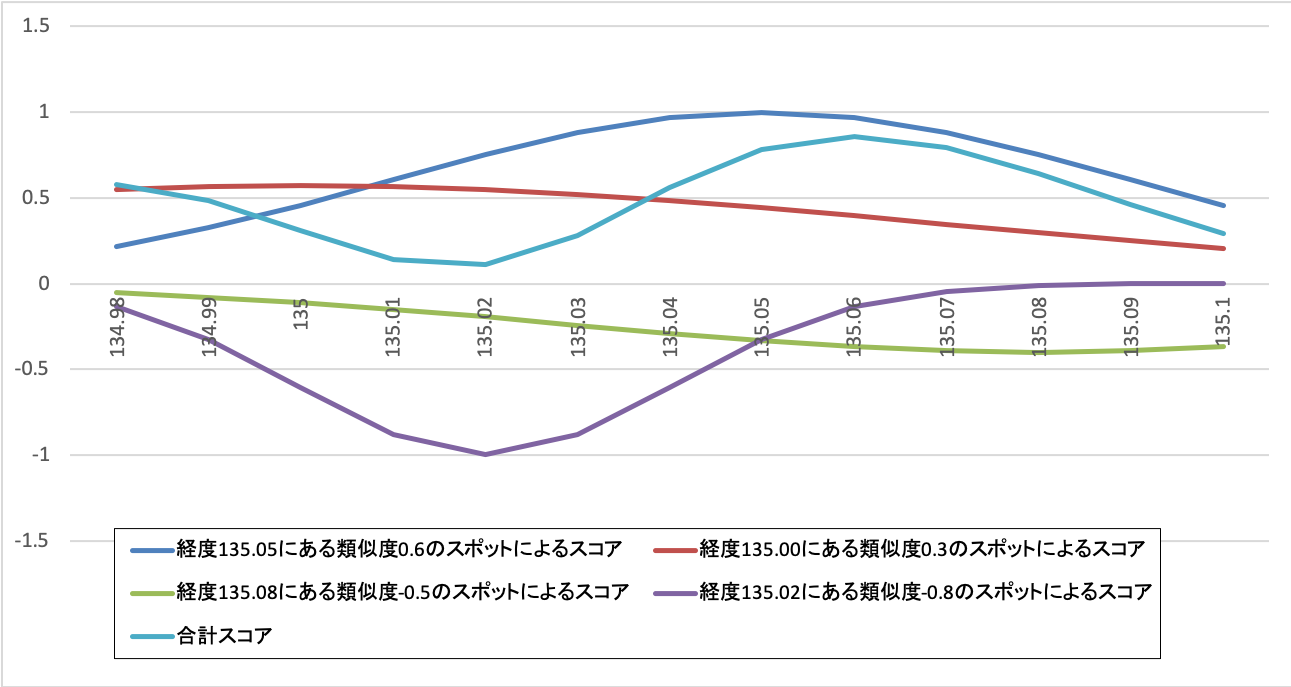
\includegraphics[clip,width=7.5cm]{picture/score_image2.png}
    \caption{既訪問スポットの経度座標計算の例}
    \label{fig:latlng}
  \end{center}
\end{figure}


%%%%%%%%%%%%%%%%%%%%%%%%%%%%%%%%%%%%%%%%%%
%%%%%%%%%%%%%%%%%%%%%%%%%%%%%%%%%%%%%%%%%
\section{クラスタ分けに関する予備実験}
%%%%%%%%%%%%%%%%%%%%%%%%%%%%%%%%%%%%%%%%%%
\subsection{実験内容}
ユーザが訪問したことのある観光スポットから,ユーザの観光スポットに対する嗜好をクラスタリングする実験を行う.
まず,既訪問スポットに対する嗜好を3つ想定したデータセットを,我々が仮想的に2人分用意する.
このデータセットを用いて既訪問スポットのレビューを取得し,階層的クラスタリングによってクラスタを作成しスコア付けを行う.
そのあと,スコア上位のクラスタを構成するレビューを分析し,想定した嗜好を含むクラスタが作成されているかどうかを確認する.

本実験を利用するデータセットの内容を以下に示す.
ユーザAのデータセットを表\ref{table:ユーザAの既訪問スポット履歴},ユーザBのデータセットを表\ref{table:ユーザBの既訪問スポット履歴}のように用意した.
ユーザAは「初詣」,「タワー」,「生物」を観光スポットに対する嗜好と仮定したユーザを想定している.
ユーザBも同様に,「遊園地」,「神社」,「山」を観光スポットに対する嗜好とするユーザを想定した.
また,ユーザの観光スポット訪問履歴には様々な嗜好が混じっていることから,「その他」として異なるジャンルの観光スポットをそれぞれ1つずつ含めている.

\begin{table}[t]
    \caption{ユーザAの既訪問スポット履歴}
    \label{table:ユーザAの既訪問スポット履歴}
    \centering
    \begin{tabular}{l|l|r}
    \hline
    \multicolumn{1}{c|}{既訪問スポット} & \multicolumn{1}{c|}{想定した嗜好} & \multicolumn{1}{c}{レビュー数} \\ \hline
    成田山新勝寺                       & 初詣                          & 787                       \\
    川崎大師                         & 初詣                          & 241                       \\
    東京スカイツリー                     & タワー                         & 237                       \\
    東京タワー大展望台                    & タワー                         & 1875                      \\
    海遊館                          & 生物                          & 2874                      \\
    沖縄美ら海水族館                     & 生物                          & 3028                      \\
    新宿御苑                         & その他                         & 1147                      \\ \hline
    \end{tabular}
\end{table}

\begin{table}[t]
    \caption{ユーザBの既訪問スポット履歴}
    \label{table:ユーザBの既訪問スポット履歴}
    \centering
    \begin{tabular}{l|l|r}
    \hline
    \multicolumn{1}{c|}{既訪問スポット} & \multicolumn{1}{c|}{想定した嗜好} & \multicolumn{1}{c}{レビュー数} \\ \hline
    富士急ハイランド                     & 遊園地                         & 1328                      \\
    ユニバーサル・スタジオ・ジャパン             & 遊園地                         & 760                       \\
    高千穂神社                        & 神社                          & 135                       \\
    天岩戸神社                        & 神社                          & 228                       \\
    阿蘇山                          & 山                           & 444                       \\
    富士山                          & 山                           & 761                       \\
    新宿御苑                         & その他                         & 1147                      \\ \hline
    \end{tabular}
\end{table}

\begin{table*}[t]
    \caption{ユーザAのクラスタ分け結果}
    \label{table:ユーザAのクラスタ分け結果}
    \centering
    \begin{tabular}{c|r|l}
    \hline
    \multicolumn{1}{c|}{クラスタ} & \multicolumn{1}{c|}{スコア} & \multicolumn{1}{c}{クラスタ内の特徴語上位10件}         \\ \hline
    151                       & 0.57                     & 水槽,ジンベイザメ,水族館,魚,ジンベエザメ,迫力,サメ,泳ぐ,沖縄,イルカショー  \\
    134                       & 0.56                     & 東京タワー,展望台,夜景,スカイツリー,東京,景色,タワー,シンボル,展望,見える  \\
    195                       & 0.14                     & 成田,成田山,うなぎ,お寺,新勝寺,成田山新勝寺,初詣,参道,節分,成田駅      \\
    155                       & 0.07                     & 記入,館内,エスカレーター,残念,従業員,悪さ,対応,お天気,コーナー,水族館    \\
    186                       & 0.06                     & 川崎大師,渡す,お祓い,バッグ,仲見世通り,御籤,一服,なんだか,APEC,すれ違う \\ \hline
    \end{tabular}
\end{table*}

\begin{table*}[t]
    \caption{ユーザBのクラスタ分け結果}
    \label{table:ユーザBのクラスタ分け結果}
    \centering
    \begin{tabular}{c|r|l}
    \hline
    \multicolumn{1}{c|}{クラスタ} & \multicolumn{1}{c|}{スコア} & \multicolumn{1}{c}{クラスタ内の特徴語上位10件}                       \\ \hline
    131                       & 0.38                     & 絶叫,アトラクション,乗れる,トーマスランド,乗り物,乗る,ええじゃないか,ジェットコースター,ドドンパ,遊園地 \\
    80                        & 0.23                     & 富士山,火口,合,登る,五合,山頂,ガス,阿蘇,阿蘇山,見える                          \\
    56                        & 0.14                     & 天岩戸,宮,高千穂峡,高千穂,神社,西本,杉,天安河原,社務所,天岩戸神社                    \\
    53                        & 0.08                     & 参拝,詣る,参拝者,あまる,うんざり,ひとつだけ,事情,仏閣,巫女,手水舎                    \\
    54                        & 0.07                     & 神話,一回り,学べる,宮崎市内,気象観測,津,美美,駅そば,かけて,説明                     \\ \hline
    \end{tabular}
\end{table*}

\subsection{実験結果と考察}
表\ref{table:ユーザAのクラスタ分け結果}と表\ref{table:ユーザBのクラスタ分け結果}は正規化ジニ分散指標とスポット数による重み付けを用いたスコア付けの結果となっている.
階層的クラスタリングによるクラスタ分類がうまく出来ているかを判断するため,スコアが大きい上位5件を取り上げて考察する.
それぞれのクラスタ内のTFIDF法で計算したTFIDF値の上位の10件の単語を抽出して,クラスタがうまく作成されているかどうかを判断する要素として利用する.

ユーザAのクラスタ分類の実験結果(表\ref{table:ユーザAのクラスタ分け結果})から,195番のクラスタでは「初詣」に関する特徴語,134番のクラスタでは「タワー」に関する特徴語,151番のクラスタでは「生物」に関する特徴語が抽出されており,我々が仮定した嗜好に合うクラスタ分類ができている.
同様に,ユーザBのクラスタ分けの実験結果(表\ref{table:ユーザBのクラスタ分け結果})から,131番のクラスタでは「遊園地」に関する特徴語,56番のクラスタでは「神社」に関する特徴語,80番のクラスタでは「山」に関する特徴語が抽出されており,我々が仮定した嗜好に合うクラスタ分類ができている.
この結果から,クラスタの構成スポット数による重み付けが,ユーザの観光スポットに対する嗜好の抽出に有用であることがわかった.
また,クラスタのスコアを見ると,スコア値が0.1以上のときには,クラスタの特徴語がうまく抽出されているに対し,スコア値が0.1より小さいときには,抽出された単語のばらつきが大きくなっている.
そのため,ユーザのに提示するクラスタはスコア値0.1以上の上位3件とする.
ユーザがスポット検索を行う際に,自分の嗜好に合うクラスタを選択することによって,より検索結果の対応付けを詳細にすることが可能だと考えられる.


% %%%%%%%%%%%%%%%%%%%%%%%%%%%%%%%%%%%%%%%%%%
% %%%%%%%%%%%%%%%%%%%%%%%%%%%%%%%%%%%%%%%%%
% \section{スポット間の対応関係に関する評価}
% %%%%%%%%%%%%%%%%%%%%%%%%%%%%%%%%%%%%%%%%%%
% \subsection{実験内容}
% 提案手法を他の手法と比較して評価を行う.
% 以下の2つの手法を使って比較する.
% \subsection{実験結果と考察}


%%%%%%%%%%%%%%%%%%%%%%%%%%%%%%%%%%%%%%%%%%
%%%%%%%%%%%%%%%%%%%%%%%%%%%%%%%%%%%%%%%%%%
\section{まとめと今後の課題}
\label{sec:まとめと今後の課題}

本研究では,ユーザが行きたい観光スポットが決まっていない場合に,ユーザの事前知識が不足しているため,観光検索サイトを使用してランキング,おすすめ情報やカテゴリなどを基に検索された観光スポットに対する理解が困難であることに着目した.
検索結果スポットに対する理解を支援するために,検索結果スポットをユーザがすでに訪れたことがある既訪問スポットと比較することによって,理解を支援する説明手法を提案した.
具体的に,ユーザの既訪問スポットから各スポットのレビューを全て取得し,そのレビューを用いて階層的クラスタリングを行った.
次に,得られたクラスタに対しユーザの嗜好を表しているかどうかのスコア付けを行い,スコア上位のクラスタの特徴語をユーザに提示した.
本稿ではシステムの実装に向けて,既訪問スポットからユーザの嗜好推定が可能かどうかについて実験を行った.
その結果,スコア上位のクラスタはユーザの嗜好を表していることが判明した.

今後の課題は,システムのインターフェースの作成およびユーザの観光スポット検索を詳細化できるか明らかにすることである.詳細化できるかを明らかにするために,提案手法と既存手法との比較実験を計画している.

%%%%%%%%%%%%%%%%%%%%%%%%%%%%%%%%%%%%%%%%%%
\section*{謝辞}
%%%%%%%%%%%%%%%%%%%%%%%%%%%%%%%%%%%%%%%%%%
本研究の一部は,2019年度科研費基盤研究(B)(課題番号:19H04118)によるものです.ここに記して謝意を表すものとします.

%%%%%%%%%%%%%%%%%%%%%%%%%%%%%%%%%%%%%%%%%%
% 文献 Reference
%%%%%%%%%%%%%%%%%%%%%%%%%%%%%%%%%%%%%%%%%%
\vspace{2em}
\begin{thebibliography}{99}
  \bibitem{Gentner}
    D. Gentner,
      ``Structure-Mapping: A Theoretical Framework for Analogy'',
      Cognitive Science, Vol.7, pp.155–170, 1983
  \bibitem{Holyoak}
    K. J. Holyoak and P. Thagard,
      ``Mental Leaps: Analogy in Creative Thought, MIT Press'',
      Journal of Japanese Society for Artificial Intelligence,  Vol.11, No.3,  pp.489, 1996
  \bibitem{Gick}
    M. L. Gick and K. J. Holyoak,
      ``Analogical Problem Solving'',
      Cognitive Psychology, Vol.12, pp.306–355, 1980
  \bibitem{潘DEIM}
    潘 健太, 北山 大輔:
      ユーザの既訪問スポットの位置付けに基づく検索結果スポットの説明手法,
      第11回データ工学と情報マネジメントに関するフォーラム(DEIM Forum 2019), H7-2, 2019
  \bibitem{潘STI}
    潘 健太, 北山 大輔:
      地図上における検索結果スポットの説明性向上のための観光スポットの対応関係可視化手法,
      観光情報学会 第20回研究会, pp.1-4, 2019
  \bibitem{Kurashima}
    T. Kurashima, T. Iwata, G. Irie and K. Fujimura.,
      ``Travel route recommendation using geotags in photo sharing sites'',
      CIKM '10 Proceedings of the 19th ACM international conference on Information and knowledge management, pp.579-588, 2010
  \bibitem{Kitamura}
    Kitamura, R. and Itoh, T.:
      Tourist Spot Recommendation Applying Generic Object Recognition with Travel Photos,
      In 2018 22nd International Conference Information Visualisation, pp.1-5, 2018
 \bibitem{櫻川2015}
    櫻川 直洋, 廣田 雅春, 石川 博, 横山 昌平:
      ジオタグ付き写真の撮影者を在住者と観光者に分類することによるホットスポットの発見,
      第7回データ工学と情報マネジメントに関するフォーラム(DEIM Forum 2015), F6-3, 2015
  \bibitem{櫻川2016}
    櫻川 直洋, 廣田 雅春, 石川 博, 横山 昌平:
      ジオタグ付き写真を用いたイベントとその穴場スポットの発見,
      第8回データ工学と情報マネジメントに関するフォーラム(DEIM Forum 2016), H5-3, 2016
 \bibitem{上村}
    上村 幸汰, 桂井 麻里衣, 真木 勇人, 後藤 亮介:
      タグ付き画像を用いたファッションスタイルの関係性の可視化,
      第11回データ工学と情報マネジメントに関するフォーラム(DEIM Forum 2019), E8-2, 2019
  \bibitem{doc2vec}
    Quoc V. Le and Tomas Mikolov,
      ``Distributed representations of sentences and documents'',
      In Proceedings of the 31th International Conference on Machine Learning, ICML 2014, pp. 1188–1196, 2014
  \bibitem{山田}
    山田 祥輝, 北山 大輔:
      ユーザの嗜好に基づく観光スポット説明文の個人化手法,
      第11回データ工学と情報マネジメントに関するフォーラム(DEIM Forum 2019), E3-1, 2019
  \bibitem{mecab}
    T. Kudo, K. Yamamoto and Y. Matsumoto,
      ``Applying Conditional Random Fields to Japanese Morphological Analysis'',
      Proceedings of the 2004 Conference on Empirical Methods in Natural Language Processing (EMNLP-2004), pp.230-237, 2004
\end{thebibliography}

\end{document}
